\begin{figure}
\begin{center}
    \centering
    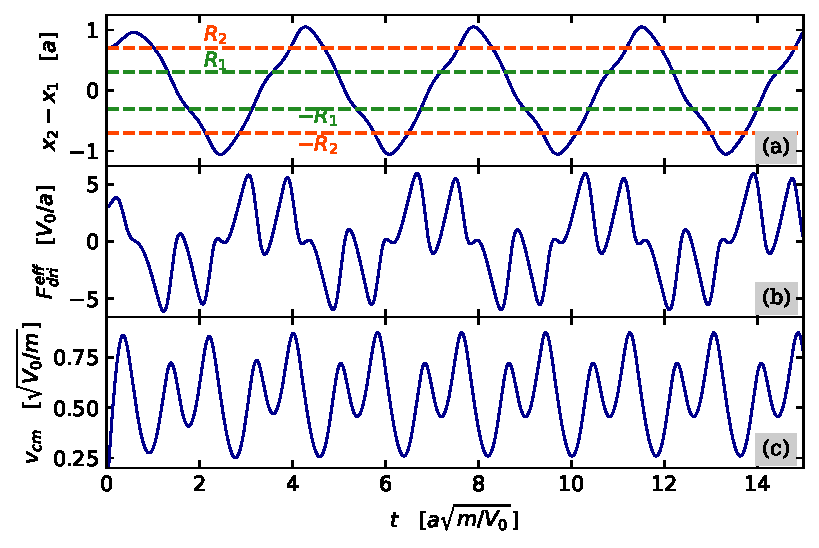
\includegraphics[width=1\linewidth]{Images/Underdamped.pdf}
    \caption{Oscillations in the underdamped case with $R_1 = 0.3 a$, $R_2 = 0.7 a$, $F = 2.6 \f$, $\gamma = 2 \g$, $ U = 1 \p$ ($\delta = 3.1999 \times 10^{-2} V_0$) and initial condition $R_0=R_2$. \textbf{(a)} relative coordinate $r$; \textbf{(b)} effective driving force $F_\text{dri}^\text{eff}$; \textbf{(c)} velocity of the center of mass $v_\text{cm}$. }
    \label{Fig:Underdamped}
\end{center}
\end{figure}

\begin{figure}
\begin{center}
    \centering
    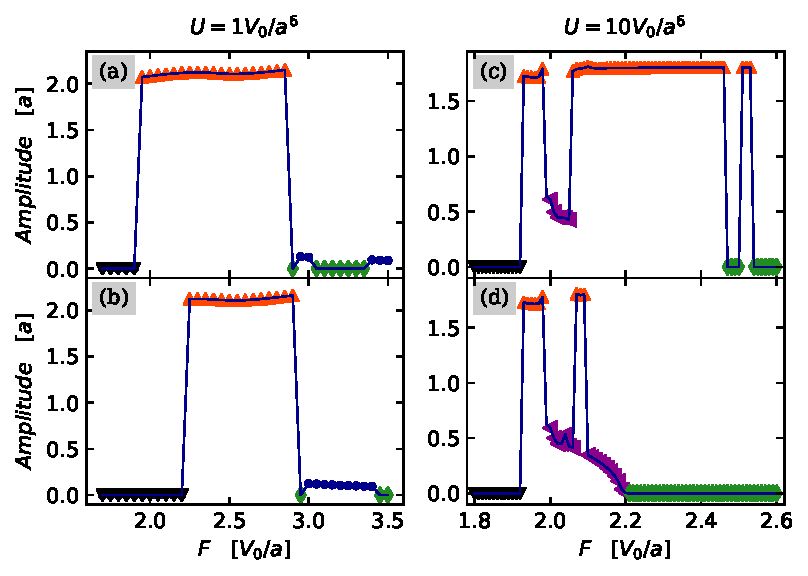
\includegraphics[width=1\linewidth]{Images/Underdamped_res_col.pdf}
    \caption{Oscillation amplitude $r_{max}-r_{min}$  as a function of $F$ for $R_1 = 0.3 a$, $R_2 = 0.7 a$, $\gamma = 2 \g$. \textbf{(a,b)}:  $ U = 1 \p$ ($\delta = 3.1999 \times 10^{-2} V_0$); \textbf{(c,d)}:  $ U = 10 \p$ ($\delta = 0.31999  V_0$). In panels \textbf{(a,c)} the initial condition is $R_0=R_2$; in panels \textbf{(b,d)} $R_0=a$. The red up-triangles mark oscillations with amplitude $A > 2R_2$, the green diamonds mark a collapse to the origin, and the purple left-triangles indicate an oscillation around the origin.}
    \label{Fig:Underdamped_res}
\end{center}
\end{figure}

\begin{figure}
\begin{center}
    \centering
    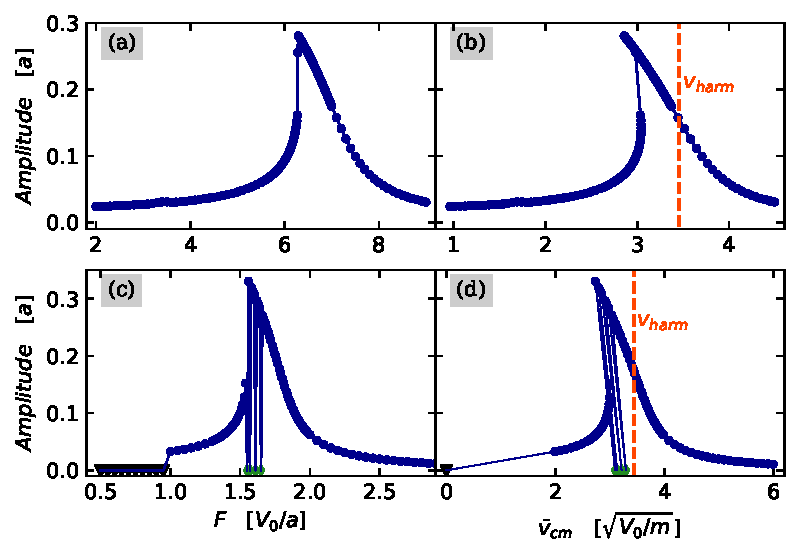
\includegraphics[width=1\linewidth]{Images/Underdamped_res_2_col.pdf}
    \caption{Effects of changing $U$ and $\gamma$. Amplitude of the oscillations for $R_1 = 0.3 a$, $R_2 = 0.7 a$, $ U = 100 \p$ ($\delta = 3.1999  V_0$) and initial condition $R_0=R_2$ and \textbf{(a,b)}: $\gamma = 2 \g$; \textbf{(c,d)}: $\gamma=0.5 \g$.}
    \label{Fig:Underdamped_res_2}
\end{center}
\end{figure}

\begin{figure}
\begin{center}
    \centering
    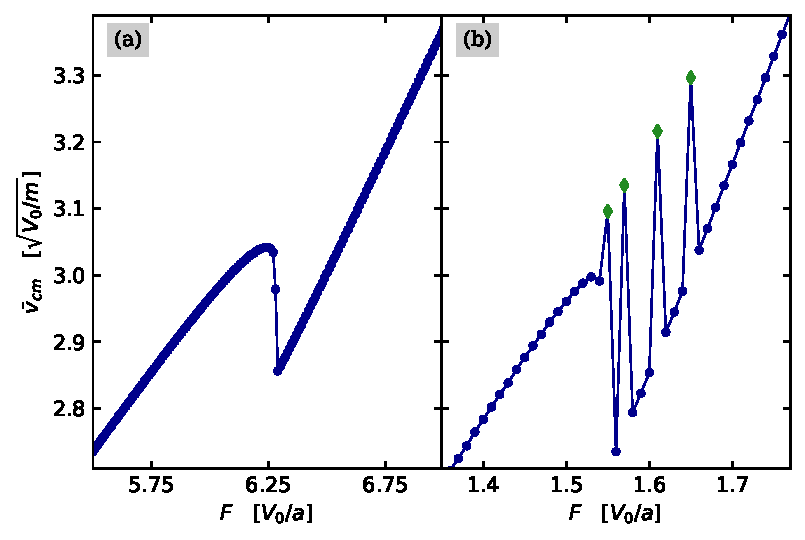
\includegraphics[width=1\linewidth]{Images/Bistability_2.pdf}
    \caption{Bistabilities of the underdamped dynamics. \textbf{(a)} Same parameters as Fig.~\ref{Fig:Underdamped_res_2} (a,b); \textbf{(b)} same parameters as Fig.~\ref{Fig:Underdamped_res_2} (c,d). The green diamonds mark a collapse at the origin.  }
    \label{Fig:Bistability}
\end{center}
\end{figure}


So far we focused on overdamped dynamics. In this section, we provide a brief overlook of the behavior of the underdamped molecule, keeping in mind that this regime is less likely to be relevant in practice. 

As shown in Fig.~\ref{Fig:Underdamped}, if $\delta$ is moderate and for small external forces $F$, a small damping produces very wide oscillations and an extremely short initial transient. The main novelty of the underdamped case is that $r$ can pass through zero without collapsing permanently there. This is possible because when $r$ passes trough the origin it carries enough momentum to escape the $r=0$ basin even if $F_\text{dri}^\text{eff}$ vanishes. Figure~\ref{Fig:Underdamped}b shows that $F_\text{dri}^\text{eff}$ vanishes every time that $r$ passes trough $0$ or $\pm a$ due to the term $\sin\left(\frac{\pi r}{a}\right)$, plus other two times due to the normal oscillation of the $\cos\left(\frac{2\pi x_\text{cm}}{a}\right)$ term. This results in a fairly intricate time dependence of $F_\text{dri}^\text{eff}$, and as a consequence the oscillation of $r$ involves a complicated pattern with several Fourier components. Figure~\ref{Fig:Underdamped}c shows that $v_\text{cm}$ too is far more complicated than a simple sinusoid. Anyway the fundamental frequency of the oscillation of $r$ and of $F_\text{dri}^\text{eff}$ is still the washboard frequency $\nu_\text{cm}$. For high values of $F$ the two well-known features of steady sliding are retrieved: the collapse to the origin and the ordinary oscillations around $R_2$, or around $-R_2$, because the particles can occasionally swap during the initial transient.

\subsection{Resonances}
To  better understand the dependence of these wide oscillations on the external force, we carry out for the underdamped system the same analysis as we did in Sec.~\ref{resonances:sec} for the overdamped molecule. Here we obtain quite different results. Figure~\ref{Fig:Underdamped_res} shows that the $F$-dependence of the oscillation amplitude is more complex and discontinuous than in the overdamped case. That is because in the latter, after the depinning force, we only had regular oscillations around $R_2$, which provide a smooth resonant behaviour. Here, on the contrary, we observe the alternation of several kinds of oscillations, one of which being exemplified Fig.~\ref{Fig:Underdamped}, and that can depend crucially on the initial condition.

We can divide Figs.~\ref{Fig:Underdamped_res} (a,b) in three ranges of applied force $F$, where different kinds of oscillation occur. Starting from small $F$, in the first range the molecule does not move, i.e.\ $F$ is below the depinning force (black down-triangles). Increasing $F$, we observe a plateau of very wide oscillations with amplitude $A > 2 R_{2}$ of the kind reported in Fig.~\ref{Fig:Underdamped} (red up-triangles). For even larger forces, we retrieve either small-amplitude oscillations around $R_2$ (blue circles) or a collapse to the origin (green diamonds), resulting in a null value of the amplitude. The comparison of panel (a) with panel (b) shows that where these regions begin and end depends on the starting condition $R_0$. Figure~\ref{Fig:Underdamped_res} (c,d), where $\delta$ is larger, reports even more complicated patterns. The oscillations with a smaller amplitude that interrupt the plateau are oscillations around the origin (purple left-triangles). This is a completely new kind of oscillation, that cannot occur in the overdamped system. In some cases, these oscillations are clean periodic oscillations around a minimum, but for some values of $F$, we even observe intricate quasi-periodic patterns.

In Fig.~\ref{Fig:Underdamped_res_2} (a,b), where we increase $U$ to  $100\p$ (so that $\delta=3.1999  V_0$), we see that a resonance peak near the harmonic frequency arises.  In Fig.~\ref{Fig:Underdamped_res_2} (c,d) we decrease $\gamma$ to $0.5\g$, and we observe that the resonance peak is interrupted by a few collapses to the origin (green diamonds). That is because with such a small damping factor, near the resonance, the oscillation extends beyond $R_1$, but then the $r=0$ minimum can sometimes capture the motion, because wide oscillations across the origin are disfavoured by the high barrier $\delta$. Panels (b,d) show a dynamical bistability near the resonance, i.e.\ the same center-of-mass velocity is obtained for different values of $F$. These instabilities are shown in more detail in Fig.~\ref{Fig:Bistability}. The same result for an underdamped dimer was observed in Ref.~\cite{Fusco}. 

In general, the underdamped dynamics exhibits a larger variety of oscillations, and is far more sensitive to the initial condition than the overdamped case. 